%\RequirePackage[l2tabu, orthodox]{nag}  %Checks for older packages

\documentclass[11pt,a4paper]{article}
% \documentclass[10pt]{extreport} $ allos to make the font smaller
\usepackage[utf8]{inputenc}

\usepackage{amsmath}
\usepackage{amsfonts}
\usepackage{indentfirst}
\usepackage{amssymb}
\usepackage[font={footnotesize}]{caption} %Makes the captions small

%\usepackage{algorithm}
%\usepackage{algpseudocode}
\usepackage[linesnumbered,ruled,vlined]{algorithm2e}

%% Figures packages
\usepackage[pdftex]{graphicx}
\usepackage{float}   %Es para colocar el objeto flotante exactamente donde se ponga el comando con H
\usepackage{caption}
\usepackage{subcaption}
\graphicspath{{./graphics/}}
\usepackage{sidecap}  %Para poner figuras a los lados


\usepackage{setspace} % Needed for Pyton syntax highlight
\usepackage{listings}    % Include the listings-package, nice verbatim for code
\usepackage{color}
\usepackage{courier}


\usepackage{cleveref} %puts figure and equation appropiately \cref{}

\usepackage{natbib} %For bibliography
%\usepackage{cite}
\usepackage{framed} % To use boxes, or frames around text

\usepackage{parskip} %Para saltos entre parrafos
\setlength{\parindent}{0pt}
\setlength{\parskip}{\baselineskip}
\usepackage[a4paper,margin=0.8in]{geometry}  %%Cambiar los margenes

\newcommand{\HRule}{\rule{\linewidth}{0.5mm}}
\newcommand{\Wb}{\mathbf{w}}

\usepackage{hyperref} %This should be loade after most of the other packages
% \hypersetup{colorlinks=true}

% Command for argmin
\DeclareMathOperator*{\argmin}{\arg\!\min}

\definecolor{dkgreen}{rgb}{0,0.6,0}


\begin{document}

\begin{titlepage}
\begin{center}
%\includegraphics[width=0.15\textwidth]{logo}\\[1cm]

\textsc{\LARGE Kungliga Tekniska Högskolan}\\[1.0cm]

\textsc{\Large Introduction to GPU and accelerator programming for scientific computing}\\[2.0cm]



\begin{figure}[H]
	\centering
 
\includegraphics[width=0.35\textwidth]{Kth_logo.png}
\end{figure}
%\\[1cm]
%

% Title
\HRule \\[0.4cm]
{ \huge  Project: Optimizing Stochastic Gradient Descent with cuBLAS.
}\\[0.4cm]
\HRule \\[1.5cm]

% Author and supervisor

Author: Theodoros Vasiloudis   \\

\textsc{\Large School of Computer Science and Communication}\\ [1.0cm]
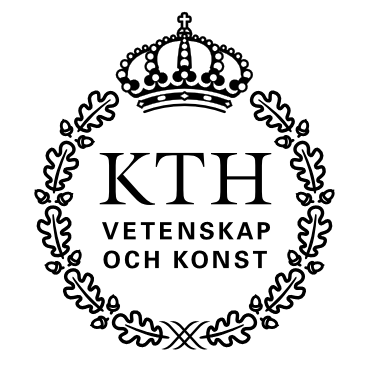
\includegraphics[width=0.15\textwidth]{KTH_black.png}\\[1.5cm] % Controls the distance till the new object
% Bottom of the page
{\large \today}

\end{center}
\end{titlepage}

\begin{abstract}
For this project we improved an existing implementation of a parallel version of the mini-batch
Stochastic Gradient Descent optimization algorithm on a GPU, using
CUDA and the Thrust and cuBLAS libraries. We examine the scale of improvements
we are able to get by using optimized BLAS calls for the GPU compared to unoptimized CUDA calls, and perform
some large scale experiments to examine the behavior of the two approaches
under different scenarios.

\end{abstract}

\section{Introduction}
\label{sec:introduction}

As our project for the PDC Summer School in High Performance Computing we implemented mini-batch
Stochastic Gradient Descent (SGD) using CUDA and the Thrust library. In that work,
we identified a few areas that we could specifically improve in our conclusions:

\begin{enumerate}
	\item \textbf{Dynamic Parallelism - cuBLAS for vector operations}
	
	SGD involves a number of vector operations, mostly dot products.
	In the current implementation these are done sequentially through \texttt{for} loops within kernels.
	By using dynamic parallelism and specifically cuBLAS operations
	we can significantly speed up these computations.
	
	
	\item \textbf{Sequential memory access}
	
	In SGD one commonly shuffles the dataset in memory before each iteration, as it has been shown to improve
	convergence performance. In the current implementation we emulate this shuffling by randomizing the
	order in which we access elements of the dataset, leading to non-sequential memory 
	accesses. What we could do instead is to shuffle the data on the GPU memory and perform 
	sequential memory accesses.
	
	\item \textbf{Change parallelism unit}
	
	In the current implementation our unit of parallelization is the size of the batch; we run one batch 
	at a time and parallelize
	the computations in terms of the data points within the batch. Common batch sizes range from 10 - 1000
	making this way to parallelize highly inefficient on the GPU, even if dynamic parallelism is employed.
	We could change the parallelism scheme of the algorithm so we can run multiple
	batches in parallel, thereby greatly increasing the parallelism and achieving much 
	higher occupancy on the GPU.
\end{enumerate}

In this project we focused on improvements 1 and 2, and slightly extended the scope of improvement 1,
to make use of matrix-vector BLAS operations instead of only vector-vector.

For improvement 1, we developed a completely new codepath for the iterations inside the SGD algorithm,
(lines 3-9 in Algorithm \ref{algo:sgd-gpu}) that uses matrix-vector operations through the cuBLAS library.
We also made changes to the old  implementation to allow us to use vector-vector cuBLAS calls from within kernels using 
dynamic parallelism.

Improvement 2 came as a pre-requisite for the new codepath that makes use of matrix-vector operations,
as BLAS routines assume that matrices lie in contiguous memory areas. To achieve that efficiently and to avoid
having to perform expensive host-device copies at each iteration, we copy the complete dataset to the GPU
once, and then shuffle it on the GPU at the start of each iteration.

The changes discussed in improvement 3 would require radical changes to the codebase which were beyond the scope
of this project, and as such were not implemented.

We investigated the performance consequences that each of the improvements brought, and extended our previous
experiments to include larger datasets that better investigate the performance of the implementations at scale.

The rest of this report is laid out as follows: Section \ref{sec:sgd} provides some theoretical background
on the algorithm used. Section \ref{sec:psgd} focuses on parallel versions of the algorithm, providing some
relevant work, and a description of the algorithm we implemented. In Section \ref{sec:improvement} we describe
the main contributions of this work, focusing on how we expect each to improve upon the original implementation.
In Section \ref{sec:results} we show an experimental evaluation of the improvements made, and in Section \ref{sec:discussion}
we discuss and analyze the results.

Readers already familiar with parallel SGD and our previous implementation are free to skip to Section \ref{sec:improvement}
where we present the main contributions of this work.

\section{Stochastic Gradient Descent}
\label{sec:sgd}


One of the most common problems in estimation, optimization theory and machine learning is
minimizing an objective function \cite{bottou2010large}. Consider the \textit{loss} function $Q(z,
\Wb)$. This function depends both on a sample $z=(x, y)$ which is a pair made of an input $x$ and an
output $y$ and on the vector $\Wb$ which parametrizes the function that connects the input to the
output.
In such a context then we would like to find the vector $\Wb$ that minimizes this error averaged
over our data. We can then write the following:

\begin{equation}
E(\Wb) = \frac{1}{n} \sum_{i=1}^n Q(z_i, \Wb)
\end{equation}

where $i$ the sample index, as we go through the complete dataset $\mathbf{z}$.

The Gradient Descent method proposes moving in the direction that minimizes the loss function order to
find $\Wb$. That is, we perform steps of a given size in the direction of the loss function gradient
and update $\Wb$ at every step:

\begin{equation}
\Wb_{t + 1} = \Wb_t - \gamma \frac{1}{n} \sum_{i=1}^n \triangledown_w Q(z_i, \Wb)
\end{equation}

where $\gamma$ controls the step size. This quantity is usually called the learning rate and
controls the rate by which we change $\Wb$. The parameter $\gamma$ is of crucial importance for the
convergence or divergence of the algorithm. Setting it too high means taking large steps 
on the error surface at each iteration,
making it possible for the algorithm to diverge. If we set $\gamma$ too small the algorithm
will not perform enough exploration, leading to slow convergence.

Under sufficient regularity assumptions when the initial estimate of $\Wb$ is close enough to the
minimum and the learning rate is small enough this algorithm can achieve linear convergence
\cite{dennis1996numerical}.

Stochastic Gradient Descent is a variation of the scheme proposed above that can be used
when the complete dataset is not available at runtime, e.g. in a streaming setting,
or when the data does not fit into memory.
In this case instead of taking the average gradient over the complete data we only use the local
gradient taken from a single datapoint to calculate the direction of movement, and update the
weights accordingly:

\begin{equation}
\Wb_{t + 1} = \Wb_t - \gamma  \triangledown_w Q(z_i, \Wb)
\end{equation}

It follows from the algorithm that this optimization can be implemented online due to the fact that
very little memory is needed for the calculation. The convergence of SGD is granted
in  some mild conditions when the learning rate $\gamma$ decreases over time in such a way that the
series  indexed by them does not diverge \cite{bottou2010large}.

In \cite{wilson2003general} it is shown, perhaps counter-intuitively, that batch gradient descent has
worse run-times and convergence characteristics when compared to stochastic gradient descent.

Mini-batch stochastic gradient descent lies somewhere in the middle between these two algorithms.
There, the optimization process is performed on small subsets of the complete dataset that are
called \textit{batches}. At each step in the algorithm we choose a random subset of the data,
calculate the gradient, and update the weights, based on the information we are able to get from
the batch. However, the as the batch size increases we get noisier estimates of the true gradient,
leading to slower convergence rate of $O(1/\sqrt{bT} + 1/T)$, where $T$ is the number of iterations
and $b$ is the size of the batch.

The main advantage in speed for mini-batch SGD comes from the fact that instead of the
vector-vector multiplications that are necessary in plain SGD, we are able to batch samples
together and perform vector-matrix multiplications, allowing us to use optimized implementations
of such operations e.g. BLAS (Basic Linear Algebra Subprograms) \cite{lawson1979basic}.

\section{Parallel Stochastic Gradient Descent}
\label{sec:psgd}
\subsection{Related Work}

There exist a number of approaches for parallelizing SGD \cite{zinkevich2010parallelized,
recht2011hogwild, dekel2012optimal}, and each comes with some advantages and disadvantages. Some of
these algorithms are mostly intended to be used in a distributed setting, but can however be
adapted to function well in a highly parallel setting as well.

The approach presented in \cite{zinkevich2010parallelized} is an intuitive parallel extension of
SGD, where each processor solves a local SGD problem using a random partition of the
complete dataset, and the solutions from each processor are then communicated and averaged. This
approach involves practically no communication between the processors during the optimization
phase. While this is beneficial in terms of network/communication costs, it results in subpar
performance when it comes to the optimality of the solution.

\cite{recht2011hogwild} also propose an asynchronous algorithm which is aimed at problems with
sparse parameters, i.e. we assume that the cost function we are optimizing can be decomposed (to a
degree). This property makes it possible for individual processors to work on different parts of
$\Wb$, and perform gradient descent using only a single parameter from the complete weight vector,
making it possible to atomically update that single parameter, in parallel with the other
processors, without the need for locking the weight vector while one processor makes its updates.
While this approach allows for fast iterations since each processor can work and update his part of
the solution independently from the others, it has the additional assumption of problem sparsity
and the lack of communication between processors can often lead to diverging solutions
\cite{dai2015analysis}.

\cite{dekel2012optimal} show a distributed mini-batch SGD approach which they show is optimal in
terms of the \textit{optimality gap} which they define as the difference between the loss given by
the optimal weight vector $Q(z, w^*)$ and the approximation obtained by the algorithm, $Q(z,
\bar{w})$. The algorithm proposed uses mini-batches to calculate approximate gradients for each
processor, which are then summed and averaged across the different processors, and the averaged
gradient is used to update the weights at the end of each iteration. While this algorithm obviously
has higher communication costs when compared to the ones we described before, it can attain better
convergence guarantees, and enjoys faster convergence in terms of number of iterations, as the
different processors have access to more up-to-date and consistent sets of weights. One drawback of
this approach when it comes to highly parallel architectures however is that its parallelization
factor is limited by the minimum of number of batches and available processors.

\subsection{Algorithm Used}

For this work we chose a variant of the algorithm described by \cite{dekel2012optimal}, which involves the following steps:

\begin{enumerate}
	\item  	For each iteration:
	\begin{enumerate}
		\item Shuffle the dataset, and split into batches of size $b$.
		\item For each batch in the dataset, do in parallel:
		\begin{enumerate}
			\item Calculate the gradient for each data point in the batch.
			\item Sum and average the gradients for all data points in the batch.
			\item Update the weight vector according to the average gradient.
		\end{enumerate}
	\end{enumerate}
\end{enumerate}

We can write the above more formally in algorithmic form:

\begin{algorithm}
	\DontPrintSemicolon % Some LaTeX compilers require you to use \dontprintsemicolon instead
	\KwIn{A dataset $\mathbf{D}$ of containing n $z=(x, y)$ items, initial learning rate $\alpha$, number of epochs $T$, batch size $b$}
	\KwOut{A vector of weights providing an approximate linear solution}
	Initialize $w$\;
	\For{$i \gets 1$ \textbf{to} $T$} {
		Shuffle the dataset, and split into $n/b$ batches\;
		\For{batch $\mathbf{z}_s$ over $\mathbf{D}$} {
			\For(\textbf{parallel}){$j \gets 1$ \textbf{to} $b$} {
				$\hat{g_j} = \triangledown_w Q(z_j, w_i)$, where $z_j \in \mathbf{z}_s$\;
			}
			$\gamma = -(\alpha / \sqrt{i}))$\;
			Do parallel sum $\sum_j{\hat{g_j}}$ to compute the average gradient for the current batch, $\bar{g_i} = 1/j \sum_j{\hat{g_j}}$\;
			Do parallel scaling of the weight vector: $w_{i + 1} = w_i - \gamma \,  \bar{g_i}$\;
		}
	}
	\Return{$w_T$}\;
	\caption{Mini-batch parallel SGD on a GPU}
	\label{algo:sgd-gpu}
\end{algorithm}

This algorithm has two differences compared to the one by \cite{dekel2012optimal}.
The first one is that where
they sum the gradients over all batches in order to reduce communication costs --the algorithm is
aimed at a distributed environment-- we are able to sum the gradient for the sample \textit{within}
each batch. We are able to do this due to the low communication costs that we have once all the
data is loaded to the GPU, and using this approach we tie the parallelization factor to the
size of the mini-batch $b$ instead of the number of batches $c$. Our assumptions were that depending 
on the data size and parameters, it may be true that $b \gg c$, allowing for better utilization of the GPU
architecture. We discussed in Section \ref{sec:introduction} why this was a bad design choice for a GPU
architecture.

The second difference is that where they take a random subset of the data at each iteration,
we have the assumption that the dataset will fit into the memory of the GPU, which allows us
to use the more traditional \textit{epochs} to train. An epoch is one pass over the complete
dataset, and by shuffling the dataset at the beginning of each epoch we are able to get better
convergence behavior as shown in \cite{bottou2010large}.

The heaviest process computationally is the gradient calculation, and it is this that we specifically targeted for our 
improvement through the use of Level 2 (matrix-vector) BLAS operations.


\section{Improvements to the original implementation}
\label{sec:improvement}

In this section we describe the implementation tools and libraries that were used in the project,
and provide an overview of the specific improvements that we made to the original implementation.

\subsection{Tools and libraries}

The tools and libraries used for this project are the following:

\subsubsection{CUDA}
The CUDA platform was first released in 2008 \cite{nickolls2008scalable} and since then it has
allowed developers and researchers to utilize the parallel computation capabilities of GPUs for scientific computing
and numerical calculations without requiring expertise on graphical programming. The CUDA API is an extension of
ANSI C, where a single operation is performed on multiple cores on the GPU in parallel, a model
that NVIDA calls SIMT for \textit{Single-Instruction-Multiple-Threads}.

The CUDA API is a low-level API, and while it provides many opportunities for optimizations, it
also requires programming in a very different paradigm than most programmers are used to, which
can lead to many errors and un-optimized implementations. For that reason we chose to use
two higher-level libraries that ease the development of programs that make use of GPUs, while
sacrificing as little performance as possible.

\subsubsection{Thrust}
Thrust \cite{bell2012thrust} is a parallel algorithms library aimed at increasing the productivity of programmers by
offering a model of programming similar to the one provided by the standard library on C++.
In other words this switches the attention from \textit{how} to compute
something to simply \textit{what} to compute. 

One of Thrust's most important features is a vector container with both host and device implementations that allow us
to use common STL operations like addition and removal of elements, as well as Thrust-specific parallel operations like \texttt{reduce}, and provides memory safety within the Thrust library.

We make use of Thrust vectors in order to store all the matrices and vectors we use
in our implementation, and use operations like \texttt{transform}, \texttt{reduce} and \texttt{reduce\_by\_key} in order to apply SAXPY operations, vector scaling, and sums.

\subsubsection{cuBLAS}

The cuBLAS library provides optimized implementations of the BLAS routines aimed at Nvidia cards.

BLAS routines provide programmers with basic building blocks for linear algebra problems, like
matrix-vector and matrix-matrix multiplication. There exist open-source implementations of these
routines such as OpenBLAS, as well as closed-source versions optimized for specific hardware such as MKL provided by Intel, and
ACML provided by AMD. cuBLAS is one such implementation provided by Nvidia that allows developers to easily
tap the processing power of GPUs in an intuitive way, without having to write CUDA code.

\subsection{Implementation of the improvements}

As mentioned in the introduction, we took a step-wise approach to the improvements made,
in order to see how each improvement affected the performance of the implementation.

Our first improvement was making very small changes to two hot-spots of the original
implementation that performed dot products between two vectors and an addition plus
scaling operation, commonly known as the AXPY operation in BLAS.
This should allow us to achieve greater utilization of the GPU, as before the kernels
were using simple \texttt{for} loops over the vectors to perform these operations.
However, since these are loops that happen over the columns (features) of the data matrix,
we can only realistically expect improvements for wide matrices with many features.

These vector-vector operations are happening within the GPU code itself, in the context of a
kernel call, so we had to use dynamic parallelism to achieve that. Dynamic parallelism
refers to the ability to launch kernels from within other kernels and is available
since CUDA version 5.0 on devices with Compute Capability $\ge$ 3.5. It's also possible
to make cuBLAS calls from within kernels which is what we did.
However as we will see in Section \ref{sec:results}, the scheduling overhead introduced by 
dynamic parallelism seems to have a huge negative effect on the overall performance.

Even without the overhead introduced by dynamic parallelism, the improvement gained from vector-vector operations
(Level 1 BLAS routines) is limited. In order to better utilize the hardware, matrix-vector (Level 2) or matrix-matrix
(Level 3) operations should be used if possible. In our case since we are dealing with a simple linear
optimization problem our model is a one-dimensional vector, which limits us to Level 2 operations.
For this we created a completely new codepath for the SGD iterations, that makes use of cuBLAS' GEMV 
(generalized matrix-vector) operations
during the gradient calculation, which is the main computational bottleneck in SGD.

Using Level 2 operations however assumes that the matrix involved is laid out in contiguous areas of the 
memory. So in order to implement this, we needed to first implement what we have listed as improvement
2 in Section \ref{sec:introduction}, namely making sure that the batches of data are laid out contiguously
in memory, and accessed in order at each iteration.

The main challenge with this improvement was that we have to shuffle the dataset at the beginning
of each iteration in order to improve convergence guarantees. This creates then a small tradeoff; compared
to the original implementation where we access data points randomly, we now have to spend extra time at the beginning of 
each iteration to shuffle the dataset in the GPU memory, so that we are able to access the data sequentially and
use the Level 2 BLAS routines. Our assumption was that the extra overhead of shuffling at each iteration would
be counteracted by the greatly increased speed in computation due to the Level 2 BLAS routines and sequential
access of the data, which was confirmed by our experiments shown in Section \ref{sec:results}. 

We use Thrust in order to perform this permutation, with the caveat that we maintain a copy of the original 
data in memory and shuffle the data by performing a permuted copy to another destination matrix/vector on the GPU.
This means that we have to use twice the amount of memory to store our data, a limitation that could be overcome
with an alternative that shuffles the data in place, but did not have the time to implement for this project.

Once we had improvement 2 in place we could proceed with creating the new codepath that utilizes
Level 2 BLAS operations to calculate the gradients. We should note that for this codepath we are not
using any CUDA device code, but rather only use either cuBLAS or Thrust calls for all the calculations, 
which we believe greatly improves the readability and maintainability of the code.

\section{Results}
\label{sec:results}

In this section we will demonstrate and briefly analyze the results of our experiments.
Since this project is about performance improvements compared
to an existing implementation, we will focus on the time it takes to run the same problem
using the different implementations. The differences between
the implementations in terms of correctness and accuracy are virtually non-existent, accounting
for numerical precision and the randomness introduced by the data shuffling.

We will show how the different implementations scale in term of the number of samples
and features in the dataset, and the size of the we set. For easy 
reference we present these parameters of interest in Table \ref{table:parameters}.


\begin{table}[H]
\centering
\begin{tabular}{|c|c|c|}
\hline
Parameter & Description & Symbol\\
\hline
Batch Size & The size of the mini batch & $b$ \\
\hline
Number of Samples & The number of training examples & $N_s$ \\
\hline
Number of Features & The number of features for each example & $N_f$ \\
\hline
\end{tabular}
\caption{Main parameters for scalability testing}
\label{table:parameters}
\end{table}

\subsubsection*{Benchmarking environment}
The experiments described below where performed on a desktop PC,
running Ubuntu 14.04 64bit. The code was compiled with CUDA version 7.5 which includes Thrust 1.8.2
and cuBLAS 7.5.18.

The hardware characteristics were: 4GB of RAM,
4-core Intel i7-870 @ 2.93Ghz (Nehalem architecture), and the GPU used was an Nvidia GTX
750Ti, a Maxwell chip (GM107) which has a Compute Capability 5.0 and comes with
4GB of GDDR5 VRAM installed.

\subsubsection*{Description of The Experiments}

In order to test our implementation of SGD we use it to estimate the weights for a linear
regression problem which can be described as follows:

\begin{equation}
	\mathbf{\hat{w}} = \argmin_{\mathbf{w}} ||\mathbf{y} - \mathbf{w}  \mathbf{X} ||^2_2
\end{equation}

that is, we try to find $\mathbf{\hat{w}}$ such that it minimizes the squared loss between
the dependent variable $\mathbf{y}$ and $\mathbf{w} \cdot \mathbf{X}$, where $\mathbf{X}$ is
our data matrix, with dimensions $N_s \times N_f$.

In order to test the performance of our program in a reliable way we 
generate our own artificial data sets. This ensures reproducibility with enough
variability and furthermore consistent access to the ground truth and 
we ensure control over $N_s$ and $N_f$ to test how our algorithm scales. 

In order to generate experiments that scale consistently  with different
data set sizes we used subsets from a bigger data set. 
That is, we first build a data set with the maximum data size that we want to 
test and then reduce it by taking pieces of arbitrary data sizes. This ensures
that the convergence characteristics of the dataset --or ``difficulty'' to learn the weights--
should be consistent across the differently sized datasets, since they originate
from the same generating process.

%In terms of accuracy we use Mean Absolute Error (MAE) as our performance criterion,
%which can be computed as follows:
%
%\begin{equation}
%	MAE = \frac{1}{N_s} \sum_1^{N_s}{|y_i - \hat{y_i}|}
%\end{equation}
%
%where $y_i$ is the true value of the dependent variable for point $i$,
%and $\hat{y_i} =\mathbf{\hat{w}} \cdot \mathbf{x_i}$ is our estimate.
%We should note that since we are interested mainly in performance in terms of running time,
%we test the algorithm on the same data we train it on, instead of having a
%separate train and test set, as is normal practice.

\subsubsection*{Experiment implementation}

In order to ease the set up and running of the experiments we used a couple of different
languages and libraries. First create the test datasets using Python and the \texttt{skcikit-learn}
library. This allows us to easily vary the size of the generated data in terms of number
of samples and features, and we are able to quickly create datasets with ranges of values.
We then use a Python script that launches the CUDA program which creates a JSON output file for each parameter setting, 
reads the results from the files, and creates the plots for the experiments.

This automated way to perform experiments allowed us to easily run our experiments, and
spend more time exploring the performance of the implementations.


\subsection{Comparison between plain CUDA and using dynamic parallelism}

For our first set of experiments we used relatively small datasets to perform comparisons
between all three implementations of the algorithm. We tested the scaling characteristics
of each in terms of number of samples, number of features and the batch size used.

For the sample number experiments we created datasets with a number of samples ranging
from 50,000 to 100,000 with 4 columns/features and used a batch size of 1000, learning rate of 0.01,
and 10 training epochs.

For the feature number experiments we created datasets with a 10,000 samples and number of features ranging
from 200 to 1,000 with and used a batch size of 1000, learning rate of 0.1,
and 20 training epochs.

For the batch size experiments we created a dataset with 100,000 samples and 1000 
and used a batch size ranging from 200 to 1200, with a learning rate of 0.1,
and 20 training epochs.


\subsubsection*{Scaling in terms of number of samples}


We will first investigate the runtime performance
of the original, plain CUDA implementation and the one using Level 1 cuBLAS
calls through dynamic parallelism.


% GPU Time for number of samples, plain CUDA vs. dynpar
\begin{figure}[H]
	\centering
	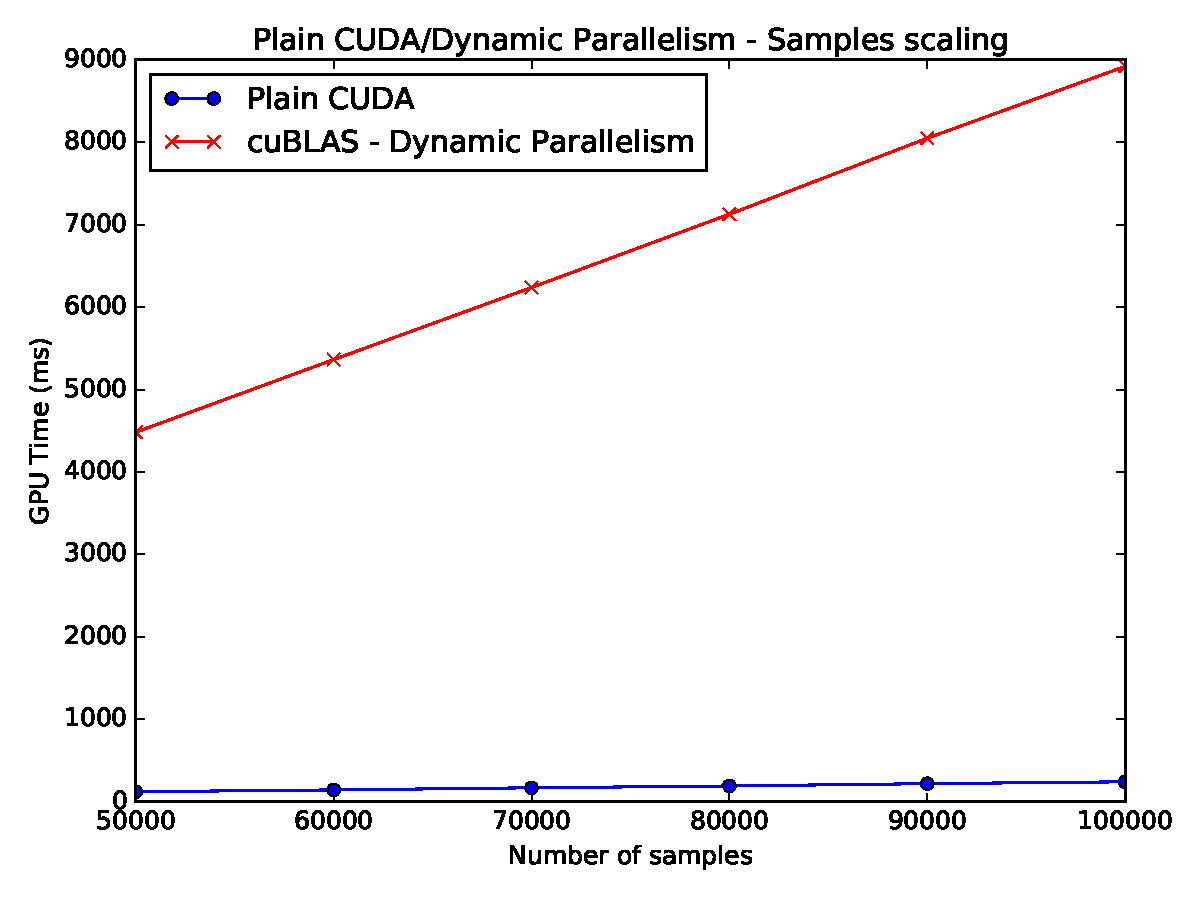
\includegraphics[width=0.8\linewidth]{gpu_plain_vs_Lvl1cuBLAS-50k-100k.pdf}
	\caption{GPU time as a function of number of samples for plain CUDA vs. cuBLAS with dynamic parallelism.}
	\label{fig:plain-dpar-n-samples}
\end{figure}

It becomes immediately evident that our use of dynamic parallelism introduces
a significant bottleneck causing the runtime to increase by two orders of magnitude.
We haven't been able to trace the source of this performance degradation, but we have
verified that our use dynamic parallelism is according to the recommendations set
by Nvidia. In our implementation as mentioned in Section \ref{sec:improvement} all
we did was change two for loops within a kernel, one to use the cuBLAS \texttt{DOT} operation
and one to use the \texttt{AXPY} operation. Our current assumption is that the scheduling
of the threads is ruined due to constant synchronization within the calling kernels.

Also, as we mentioned in Section \ref{sec:improvement}, for a small number of features like the
4 used in this experiments we don't expect any improvement as there is very little to do in parallel.
We investigate what happens when many features are used in the following experiments.

\pagebreak

\subsubsection*{Scaling in terms of number of features}

For larger number of features, the difference becomes less pronounced, but remains largely similar
as before.

% GPU Time for number of features, plain CUDA vs. dynpar
\begin{figure}[H]
	\centering
	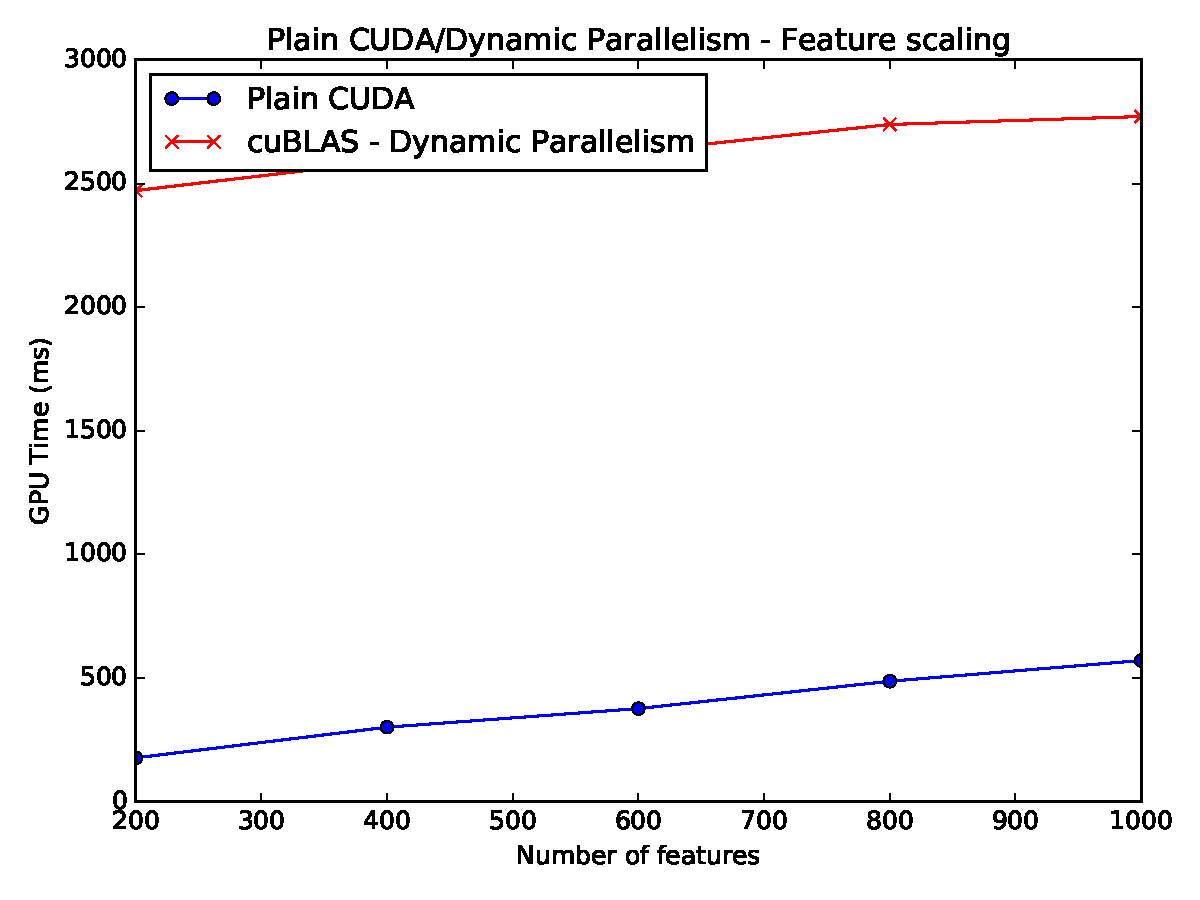
\includegraphics[width=0.8\linewidth]{gpu_plain_vs_Lvl1cuBLAS-200f-1000f.pdf}
	\caption{GPU time as a function of number of features for plain CUDA vs. cuBLAS with dynamic parallelism.}
	\label{fig:plain-dpar-n-features}
\end{figure}

With this in mind, we cannot claim that the performance degradation comes from a lack of parallelism
potential. The last potential cause we wanted to investigate was having a lack of parallelism
per block, which we do next.

\pagebreak

\subsubsection*{Scaling in terms of number of batch size}

We wanted to investigate whether the large batch size (1000) that determines the unit
of parallelism in our implementation interfered with the scheduler's ability to schedule
new threads to perform the dynamic parallelism operations. Since each block can run at most 1024 threads,
it could be possible that we were "filling" each block with the parallel threads for the batch, leaving
no threads free to run the vector operations in parallel. By using smaller batch sizes we might be able
to launch more parallel threads for the vector operations. We can see the results of these experiments
in Figure \ref{fig:plain-dpar-batch-size}.

% GPU Time for batch size, plain CUDA vs. dynpar
\begin{figure}[H]
	\centering
	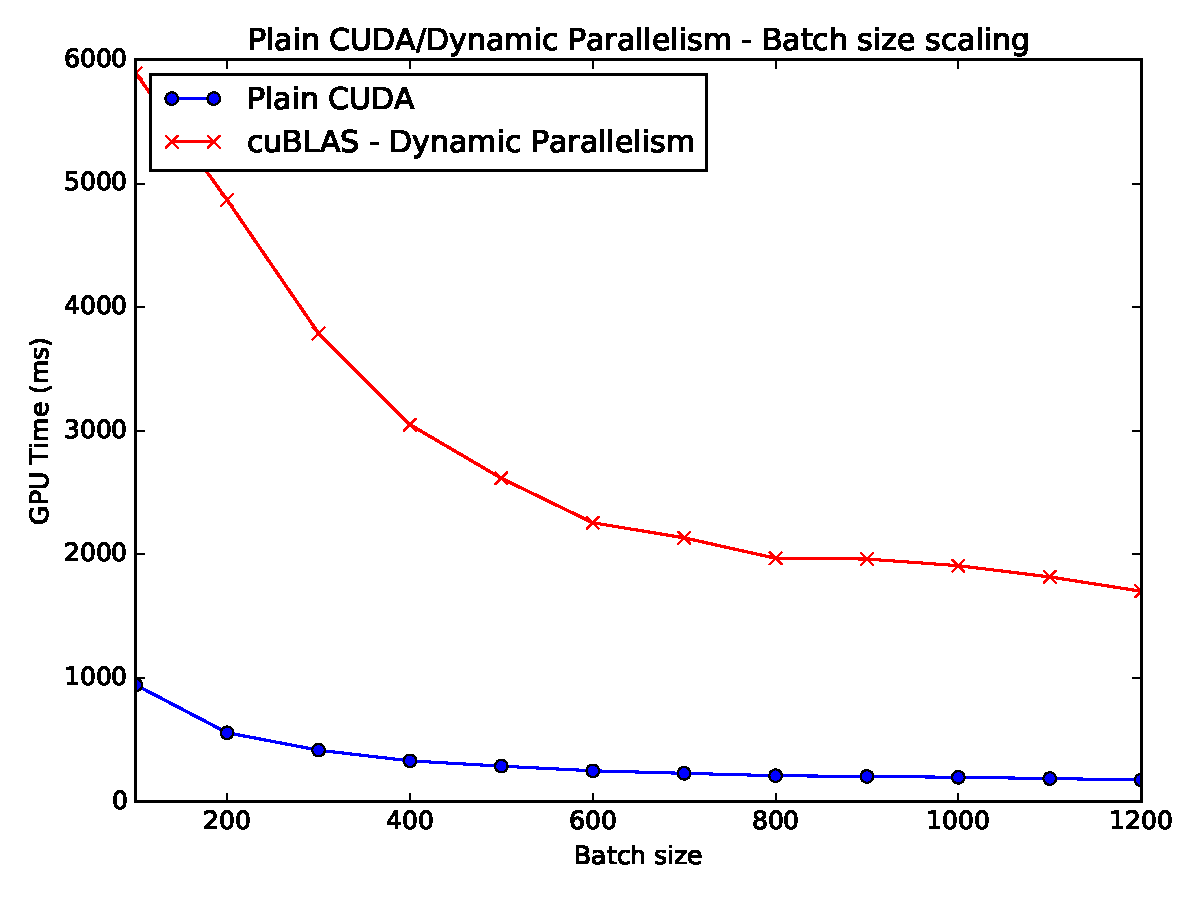
\includegraphics[width=0.8\linewidth]{gpu_plain_vs_Lvl1cuBLAS-100b-1200b.pdf}
	\caption{GPU time as a function of batch size for plain CUDA vs. cuBLAS with dynamic parallelism.}
	\label{fig:plain-dpar-batch-size}
\end{figure}

We can see in Figure \ref{fig:plain-dpar-batch-size} that as the batch size increases the difference becomes less pronounced,
but it still remains at around an order of magnitude. So with something obviously going wrong with
our implementation of dynamic parallelism, in the rest of the experiments we will focus on the differences
between our original implementation and the new one using Level 2 cuBLAS routines.

\pagebreak

\subsection{Comparison between plain CUDA and using cuBLAS Level 2 routines}

We start our comparison of the implementations using the relatively small scale datasets
we used in the previous experiments.

\subsubsection*{Scaling in terms of number of samples}

We take a look at the scaling in terms of number of samples first. Our expectation is that there shouldn't be a large difference
between the two, because given the very small number of features (4), there is not a lot of room
for the Level 2 routine to operate.

% GPU Time for number of samples, plain CUDA vs. cuBLAS
\begin{figure}[H]
	\centering
	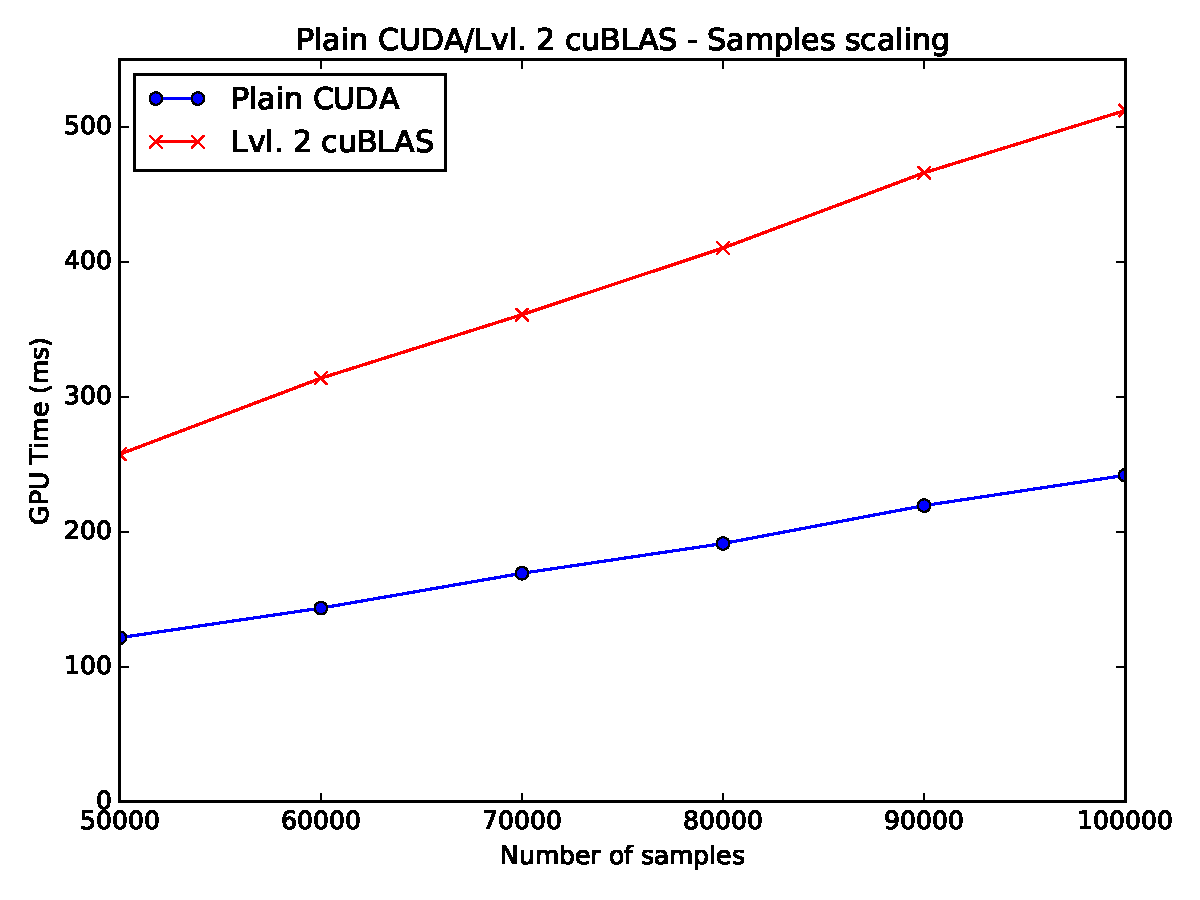
\includegraphics[width=0.8\linewidth]{gpu_plain_vs_Lvl2cuBLAS-50k-100k.pdf}
	\caption{GPU time as a function of number of samples for plain CUDA vs. Lvl. 2 cuBLAS.}
	\label{fig:plain-cublas-n-samples}
\end{figure}

Our assumptions were confirmed from the experiments as shown in Figure \ref{fig:plain-cublas-n-samples}.
The overhead introduced by the shuffling of the data and the use of the cuBLAS routine
results in longer runtimes compared to the original implementation.

We investigate what happens when large numbers of features are used in the following experiments.

\pagebreak

\subsubsection*{Scaling in terms of number of features}

For larger number of features, there should be enough level of parallelism so that
the optimized Level 2 routines can make up for the overhead introduced by the shuffling.

% GPU Time for number of features, plain CUDA vs. cuBLAS
\begin{figure}[H]
	\centering
	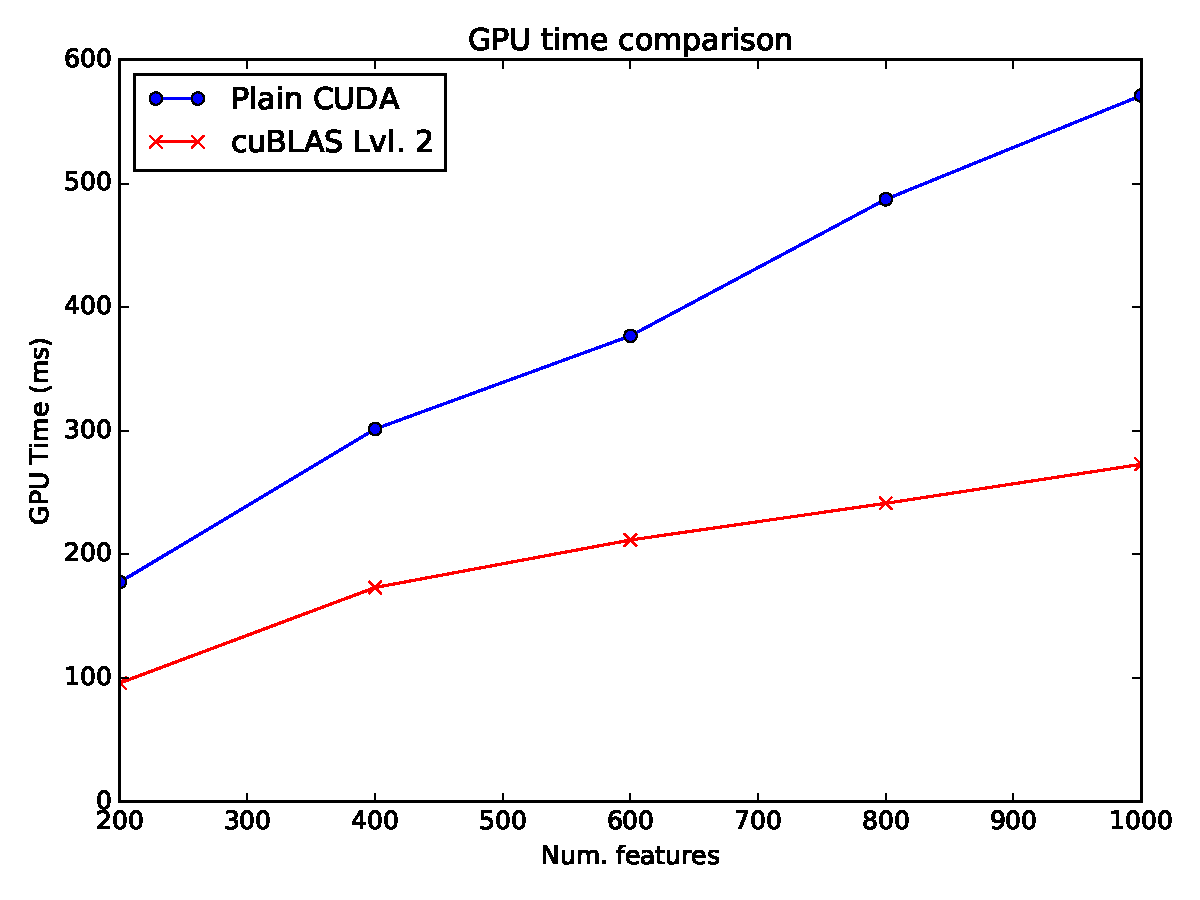
\includegraphics[width=0.8\linewidth]{gpu_plain_vs_Lvl2cuBLAS-200f-1000f.pdf}
	\caption{GPU time as a function of number of features for plain CUDA  vs. Lvl. 2 cuBLAS.}
	\label{fig:plain-cublas-n-features}
\end{figure}

Figure \ref{fig:plain-cublas-n-features} illustrates exactly that. The performance gain
from the added parallelism in terms of features allows the cuBLAS code to run approximately twice
as fast, and maintain better scaling characteristics as well (runtime increases $\sim$2x for 5x features,
vs. an increase of $\sim$3x for the original implementation for the same increase in features).

\subsubsection*{Scaling in terms of number of batch size}

For the batch size experiments we mentioned we only used 256 features to allow for parallelism "room"
for the dynamic parallelism implementation. As a result, the differences between the original
implementation and the Level 2 cuBLAS code are less pronounced, and become smaller as the batch
size increases, as shown in Figure \ref{fig:plain-cublas-batch-size}.

% GPU Time for batch size, plain CUDA vs. cuBLAS
\begin{figure}[H]
	\centering
	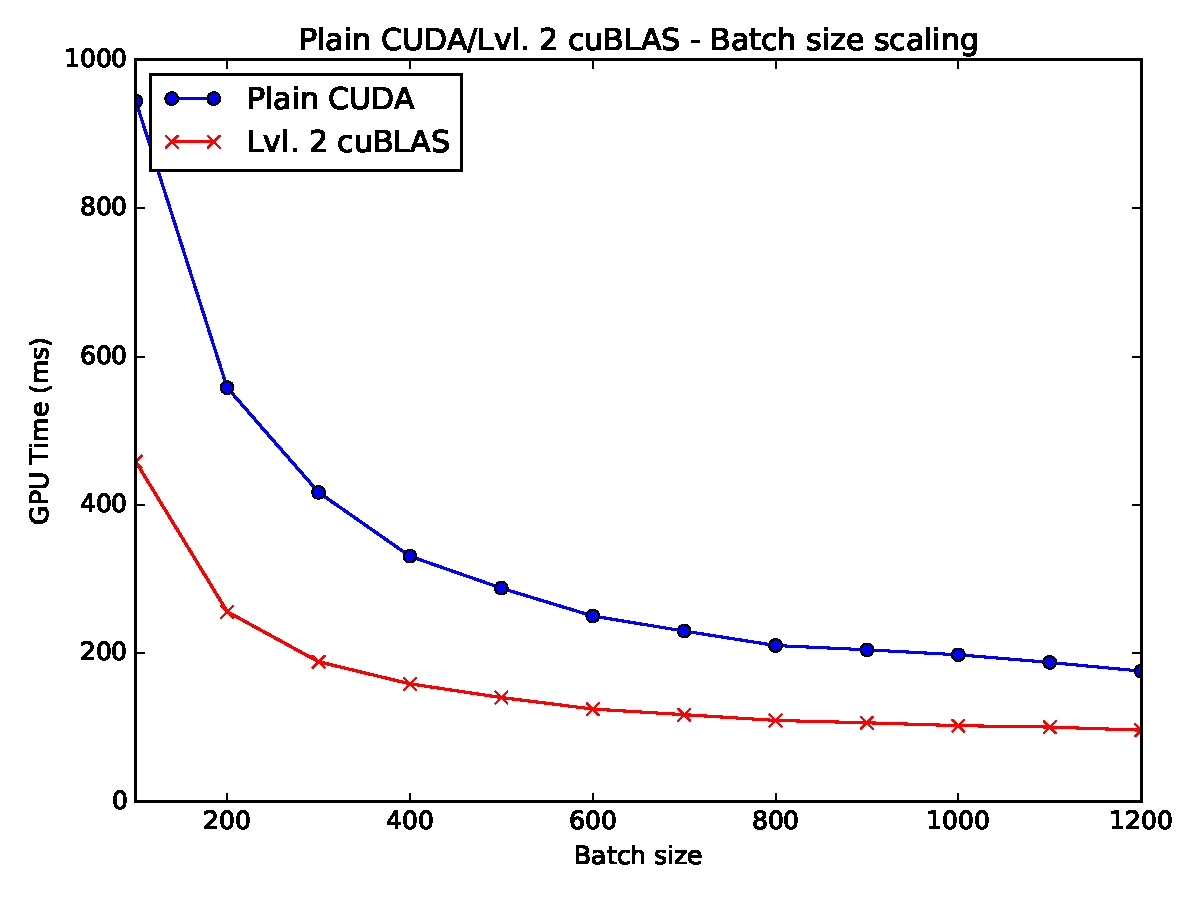
\includegraphics[width=0.8\linewidth]{gpu_plain_vs_Lvl2cuBLAS-100b-1200b.pdf}
	\caption{GPU time as a function of batch size for plain CUDA  vs. Lvl. 2 cuBLAS.}
	\label{fig:plain-cublas-batch-size}
\end{figure}

\subsection{Larger scale experiments}

After observing these performance differences, we finally wanted to investigate two things:
how do the two implementations differ when it comes to large datasets, and how does the
performance change when we change the shape of the data matrix, but keep the number of elements
the same. We summarize these results in Table \ref{table:large-scale-runtimes}:

\begin{table}[h]
	\centering
	\begin{tabular}{|c|c|c|c|}
		\hline  & $100k \times 1k$ & $10k \times 10k$ & $200k \times 2k$ \\ 
		\hline Level 2 cuBLAS & 1488.73 & 855.02 & 4417.53 \\ 
		\hline Plain CUDA & 2832.07 & 2286.13 & 20819.90\\ 
		\hline Relative difference & $\mathbf{\times1.9}$ & $\mathbf{\times2.7}$ & $\mathbf{\times4.7}$\\ 
		\hline 
	\end{tabular} 
	\caption{Comparing runtimes in $ms$ for plain CUDA and Lvl. 2 cuBLAS for large scale data.}
	\label{table:large-scale-runtimes}
\end{table}

We can see that for the same number of datapoints, as the table becomes wider the Level 2 cuBLAS
implementation has bigger gains, which is expected since the \texttt{for} loops in the original
code are performed over the columns in the dataset. The final column of the table shows that as 
the overall size of the table increases, the gains for the cuBLAS implementation become more
pronounced. We should note that at $200k \times 2k$ the size of the data table in memory becomes $\sim$1.5GB,
and with the doubling of the data size mentioned in Section \ref{sec:improvement} the memory usage
for the GPU in the cuBLAS implementation goes to $\sim$3.0GB, out of 4.0GB available in the GPU we used. If we want
our implementation to scale to bigger data sizes then an in place data shuffling method becomes necessary.

\section{Discussion}
\label{sec:discussion}

The results from using dynamic parallelism were unexpected and further investigation is needed
to determine if it is our implementation that is suboptimal, or if there is an inherent performance
penalty to using cuBLAS calls in such a manner. Using Level 2 cuBLAS calls however brought 
the performance benefits we expected, especially as we scale up to larger problem sizes.

We would like to note again that by using the Thrust and cuBLAS libraries,
we were able to implement the same algorithm without writing any CUDA code.
Our experiments show then that using high-level BLAS routines has the potential
to improve performance while at the same time simplify the code and make it
more readable and maintainable.

We believe that when the hotspots of a program are basic linear algebra routines,
achieving better performance by hand-crafted CUDA kernels is very hard without
specific assumptions about the data (like the width of the matrix), and the performance gain vs. maintainability
of the code is a tradeoff every developer has to consider but is often overlooked.
For large projects that span multiple years and developers, giving up some potential
performance for a dramatic increase in code readability and maintainability is often
the better choice.

In terms of future work we would like to continue improving this implementation
as a way to learn event more about GPU programming. As mentioned in the introduction, it suffers from the bad design
choice of using the batch size as the unit of parallelism, which is a major drawback,
and will take significant changes to the codebase to fix.
Also, in our cuBLAS code we are needlessly using twice the amount of memory needed
to hold the data, which could also be addressed without major changes to the codebase.
Another potential improvement is overlapping file IO with computation. Currently
the most time consuming part of an experiment is reading the file from disk.
If we instead overlap the reading of file chunks with running the computation
we could achieve some more time savings.


\bibliographystyle{plainnat}
\bibliography{sese_report}
\end{document}